\documentclass{article}

\usepackage{graphicx}
\usepackage{placeins}
\usepackage[utf8]{inputenc}
\usepackage{listings}
\usepackage{hyperref}
\usepackage{xcolor}
\usepackage[nodayofweek,level]{datetime}
\usepackage{ulem}
\usepackage{mathtools}

\DeclarePairedDelimiter{\ceil}{\lceil}{\rceil}

\definecolor{darkgreen}{RGB}{50,200,50}
\definecolor{verylightgray}{gray}{0.85}
\definecolor{goldenbrown}{rgb}{0.558215, 0.0, 0.135316}

\lstdefinelanguage{solidity}
{
	keywords={uint256, bytes32, mapping, address, uint40, bool, uint32, msg, sender, false, true},
	keywordstyle=\color{blue},
	keywords=[2]{pragma, contract, event, enum, struct, function, return, private, public, constant, returns, var, for, !, if, break, continue, throw, &&, ||, else, =, ==, <, >, <=, >=},
	keywordstyle=[2]\color{magenta},
	comment=[l]{//},
	commentstyle=\color{darkgreen},
	numbers=left,
	extendedchars=false,
	morestring=[b]",
	stringstyle=\color{goldenbrown},
	breaklines=true,
	backgroundcolor=\color{verylightgray},
	basicstyle=\linespread{1}\ttfamily\footnotesize
}

\title{Consensus in declarative process models using distributed smart-contracts}
\author{Mikkel Gaub, \\ Tróndur Høgnason, \\ Malthe Ettrup Kirkbro, \\ \& Mads Frederik Madsen }
\date{}

\begin{document}

\normalem
	\begin{titlepage}
		\maketitle		
		\hspace{-18pt}
		\textit{May 15, 2017}
		\vspace{\fill}
		\section*{Abstract}
		This paper investigates how efficently declarative process models can be implemented using distributed smart-contracts, more concretely the Dynamic Condition Response (DCR) engine will be implemented on the Ethereum platform, with a focus on minimizing the cost of running such an engine.
		\thispagestyle{empty}
	\end{titlepage}
	\clearpage

	\pagenumbering{arabic}
	\setcounter{page}{1}

	\tableofcontents
	\pagebreak

	\section{Introduction}

	\section{Distributed Condition Response graphs}
	A Distributed Condition Response (DCR) graph is a representation of a workflow. 
	The graph is made up of one or more activities with zero or more relations between them. 
	The following section is loosely based on a similar description in our bachelor-project \cite{bachelor}. 

	\subsection{Activity}
	The activities in a DCR graph have three attributes: included, executed and pending. 
	The attributes can be true or false. 
	Furthermore an activity can have role and actor specific execution rights.

	\subsubsection{Included attribute}
	If the include attribute of an activity is true, the activity is included and it can be executed. 
	If the attribute is false, the activity is excluded and can no longer be executed.

	\subsubsection{Pending attribute}
	If any activity in a workflow has a pending attribute that is true and the activity is included, the workflow is in an unfinished state. 
	Every time an activity is executed its pending attribute is set to false.
	This means that setting the pending attribute of an included activity to true is specifying that this activity \emph{must} be executed or excluded at some point to finish the workflow.

	\subsubsection{Executed attribute}
	If an activities executed attribute is false executing the activity will set its executed attribute to true.
	Executing an already executed activity will have no effect on the executed attribute.

	\begin{figure}[h]
		\centering
		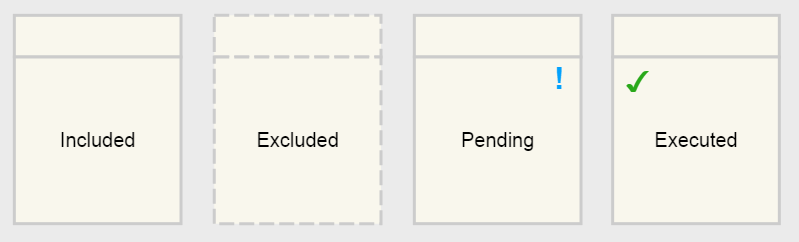
\includegraphics[width=1\textwidth]{figures/activity_states.png}
	 	\caption[Activity States]
	 	{From left to right: A visual representation of an included, excluded, pending and executed activity as presented on \href{http://www.dcrgraphs.net}{dcrgraphs.net}}.
	\end{figure}

	\subsection{Relations}
	There are five types of relations which define different types of relationships between activities in a workflow. 
	These five are the \emph{condition}, \emph{response}, \emph{include}, \emph{exclude} and \emph{milestone} relations.

	\subsubsection{Condition relation}
	If there is a condition relation from activity A to activity B, then B can only be executed if A's executed attribute is true.
	\begin{figure}[h!]
		\centering
		
\includegraphics[width=0.3\textwidth]{figures/ConditionRelation.png}
	 	\caption[Condition relation]
	 	{Condition relation}
	\end{figure}

	\subsubsection{Response relation}
	If there is a response relation from activity A to activity B, then B's pending attribute will be set to true every time A is executed.
	\begin{figure}[h!]
		\centering
		
\includegraphics[width=0.3\textwidth]{figures/ResponseRelation.png}
	 	\caption[Response relation]
	 	{Response relation}
	\end{figure}

	\subsubsection{Include relation}
	If there is an include relation from activity A to activity B, then B's included attribute will be set to true every time A is executed.
	\begin{figure}[h!]
		\centering
		
\includegraphics[width=0.3\textwidth]{figures/IncludeRelation.png}
	 	\caption[Include relation]
	 	{Include relation}
	\end{figure}

	\subsubsection{Exclude relation}
	If there is an exclude relation from activity A to activity B, then B's included attribute will be set to false every time A is executed.
	\begin{figure}[h!]
		\centering
		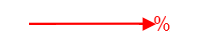
\includegraphics[width=0.3\textwidth]{figures/ExcludeRelation.png}
	 	\caption[Exclude relation]
	 	{Exclude relation}
	\end{figure}

	\paragraph{Milestone relation}
	If there is a milestone relation from activity A to activity B, then B can only be executed if A's pending attribute is false or A's included attribute is false.
	\begin{figure}[h!]
		\centering
		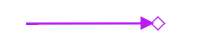
\includegraphics[width=0.3\textwidth]{figures/MilestoneRelation.png}
	 	\caption[Milestone relation]
	 	{Milestone relation}
	\end{figure}

	\subsection{Example workflow}
	Figure \ref{fig:exampleWorkflow} shows an DCR graph modeling a support ticket workflow. When the workflow is created only \texttt{Submit ticket} is executable. 
	\texttt{Close ticket} cannot be executed as it is excluded and there is a condition relation to it from an activity that is not executed. 
	\texttt{Propose solution} and \texttt{Reject solution} cannot be executed as there are condition relations to them from activities that have not been executed. 
	Lastly \texttt{Accept solution} cannot be executed as there is a milestone relation to it from \texttt{Propose solution} which is pending and not excluded.
	\begin{figure}[h!]
		\centering
		\includegraphics[width=\textwidth]{figures/exampleWorkflow.png}
	 	\caption[Example workflow]
	 	{Example workflow}
	 	\label{fig:exampleWorkflow}
	\end{figure}
	\FloatBarrier
	A typical example of an execution order of the example workflow would look like this:
	\begin{enumerate}
		\item The customer executes \texttt{Submit ticket} which excludes itself. 
		This includes \texttt{Close ticket}, but \texttt{Close ticket} is still not executable, as there is a condition relation to it from \texttt{Accept solution}.
		\texttt{Propose solution} however is now executable.
		\item The supporter executes \texttt{Propose solution}. Now \texttt{Accept solution} is executable as \texttt{Propose solution} is no longer pending and \texttt{Reject solution} is also executable as \texttt{Propose solution} is executed. 
		Furthermore \texttt{Accept solution} is now pending and must therefore be executed or excluded at some point.
		\item If the customer is not satisfied with the solution he can execute \texttt{Reject solution} which will prevent execution of \texttt{Accept solution}, as \texttt{Propose solution} is now pending and still included. 
		The workflow is now in the same state as in step 2 except from the fact that \texttt{Reject solution} is executable. 
		Executing \texttt{Reject solution} will however have no effect, as \texttt{Propose solution} is already pending.
		\item If the customer on the other hand is satisfied with the supporters solution he can execute \texttt{Accept solution}.
		Executing \texttt{Accept solution} will exclude \texttt{Propose solution} and \texttt{Reject solution}.
		This leaves \texttt{Close ticket} executable and pending.
		To leave the workflow in a finished state the supporter must execute \texttt{Close ticket}. 
	\end{enumerate}

	\section{Ethereum}
		For efficient distribution of, and consensus in, the workflows, we use the platform Ethereum. 
		Ethereum is a blockchain technology that allows for code publication and execution via the Ethereum blockchain.  
		Central for blockchain technologies is cryptocurrency, which is used to provide incentive for mining, and in Ethereum's case, to pay for computations called \textit{gas}\cite{yellow-paper}.
		Ethereum's cryptocurrency is called \textit{Ether}\cite{yellow-paper}.

		For the purposes of distribution and code execution via the Ethereum blockchain, the Ethereum yellow paper specifies a virtual machine, which achieves what the authors call "quasi-Turing-completeness"\cite{yellow-paper}. 
		They define this to be Turing-completeness, with the amount of computation bounded by the amount of gas provided,
		i.e infinite computation is impossible, since the amount of gas will always be finite. 

		\subsection{Blockchain}
		A blockchain is a distributed and decentralized database, consisting of so called \emph{blocks}\cite{bitcoin-white-paper}. 
		Each block contains the changes to the database since the last block, as well as a reference to the last block.
		To ensure that data cannot be overwritten, each block must be verified by a cryptographic puzzle, namely finding nonce to include in the block such that the hash of the block is prefixed with a number of zeroes, called the \emph{difficulty}\cite{bitcoin-white-paper}. 
		The process of finding these hashes is commonly called \emph{mining}.
		The difficulty is automatically adjusted according to the number of miners, to achieve a statistically bounded time between the publication of each subsequent block.
		Multiple blocks can be published at the same, and thus reference the same preceding block, which is called a \emph{fork} in the blockchain.
		Forks are handled slightly differently according to the specific blockchain implementation, but is generally based on some sort of the-longest-chain-wins scheme, i.e. the block most used in the system afterwards will be the block that the accepted block, while the other is rejected.
		
		Ethereum's blockchain

		\subsection{Ethereum Virtual Machine}

		\subsection{Currency}

	\section{Implementation requirements}

	All of the proposed solutions will contain the following features:
	\begin{itemize}
		\item Creation of a workflow
		\item Execution of an activity
		\item Execution rights on the level of a user and on the level of a group
		\item Visibility?
	\end{itemize}


	\section{Multi-contract implementation}

	As the gas costs of ethereum are largely dominated by the price of creating a contract, creating a contract for each activity seems unfeasible and also has security concerns related to it which will be covered later...

	The first proposed solution is creating a contract for each workflow...

	\section{Mono-contract implementation}

	The second proposed solution is creating a single contract which controls all workflows...

	\section{Comparison}
	In order to compare the solutions to each other, a simple workflow has been created modelling each of the five relations...

	\begin{description}
		\item[Contract creation]
		\item[Successful execution] ...
		\item[Failed execution] ... 
	\end{description}

	\section{Optimizations}

		\subsection{Bitfields}

		\subsection{Incoming/Outgoing}

		\subsection{etc.}


	\section{Discussion}

	\section{Further features}

		\subsection{External relations}

		\subsection{Workflow changes}

		\subsection{External contract conditions}

	\section{Vulnerabilities}

		\subsection{External relations attack}

		\subsection{Workflow updating attack}

	\section{Conclusion}

	\pagebreak
	\addcontentsline{toc}{section}{References}	
	\begin{thebibliography}{99}
	
		\bibitem{yellow-paper}
		Wood, G.
		\textit{Ethereum: A Secure Decentralised Generalised Transaction Ledger}. 
		\url{http://yellowpaper.io}.
		Accessed 2017-05-09.

		\bibitem{bachelor}
		Gaub et al.
		\textit{Consensus in peer-to-peer systems}.
		Unpublished manuscript.
		IT-University of Copenhagen,
		Denmark,
		2016.

		\bibitem{ethereum-white-paper}
		Various authors.
		\textit{White Paper}.
		\url{https://github.com/ethereum/wiki/wiki/White-Paper},
		Accessed 2017-05-09.

		\bibitem{bitcoin-white-paper}
		Nakamoto, S.
		\textit{Bitcoin: A Peer-to-Peer Electronic Cash System}.
		\url{https://bitcoin.org/bitcoin.pdf},
		Accessed 2017-05-09.


	\end{thebibliography}

	\appendix

	\clearpage

	\section{Gas prices}
		\label{app:gas-prices}

		As of May 9th, 2017, the gas prices are\cite{yellow-paper}:
		\begin{table}[h!]
		\footnotesize
		\noindent \begin{tabular}{| l | l | p{8cm} |}
			\hline
			Name 				& Value 	& Description \\ \hline
			$G_{zero}$ 			& 0 		& Nothing paid for operations of set $W_{zero}$. \\ \hline
			$G_{base}$ 			& 2 		& Amount of gas to pay for operations of the set $W_{base}$. \\ \hline
			$G_{verylow}$ 		& 3 		& Amount of gas to pay for operations of the set $W_{verylow}$. \\ \hline
			$G_{low}$ 			& 5 		& Amount of gas to pay for operations of the set $W_{low}$. \\ \hline
			$G_{mid}$ 			& 8 		& Amount of gas to pay for operations of the set $W_{mid}$. \\ \hline
			$G_{high}$ 			& 10 		& Amount of gas to pay for operations of the set $W_{high}$. \\ \hline
			$G_{extcode}$ 		& 700 		& Amount of gas to pay for operations of the set $W_{extcode}$. \\ \hline
			$G_{balance}$ 		& 400 		& Amount of gas to pay for a BALANCE operation. \\ \hline
			$G_{sload}$ 		& 200 		& Paid for a SLOAD operation. \\ \hline
			$G_{jumpdest}$ 		& 1 		& Paid for a JUMPDEST operation. \\ \hline
			$G_{sset}$ 			& 20000 	& Paid for an SSTORE operation when the storage value is set to non-zero from zero. \\ \hline
			$G_{sreset}$ 		& 5000 		& Paid for an SSTORE operation when the storage value's zeroness remains unchanged or is set to zero. \\ \hline
			$R_{sclear}$ 		& 15000		& Refund given (added into refund counter) when the storage value is set to zero from non-zero. \\ \hline
			$R_{suicide}$ 		& 24000 	& Refund given (added into refund counter) for suiciding an account. \\ \hline
			$G_{suicide}$ 		& 5000 		& Amount of gas to pay for a SUICIDE operation. \\ \hline
			$G_{create}$ 		& 32000		& Paid for a CREATE operation. \\ \hline
			$G_{codedeposit}$ 	& 200 		& Paid per byte for a CREATE operation to succeed in placing code into state. \\ \hline
			$G_{call}$ 			& 700		& Paid for a CALL operation. \\ \hline
			$G_{callvalue}$ 	& 9000		& Paid for a non-zero value transfer as part of the CALL operation. \\ \hline
			$G_{calstipend}$ 	& 2300		& A stipend for the called contract subtracted from $G_{callvalue}$ for a non-zero value transfer. \\ \hline
			$G_{newaccount}$ 	& 25000		& Paid for a CALL or SUICIDE operation which creates an account. \\ \hline
			$G_{exp}$ 			& 10 		& Partial payment for an EXP operation \\ \hline
			$G_{expbyte}$ 		& 10		& Partial payment when multiplied by $\ceil{log_{256}(exponent)}$  for the EXP operation. 	 \\ \hline
			$G_{memory}$ 		& 3			& Paid for every additional word when expanding memory. \\ \hline
			$G_{txcreate}$ 		& 32000		& Paid by all contract-creating transactions after the Homestead transition. \\ \hline
			$G_{txdatazero}$ 	& 4 		& Paid for every zero byte of data or code for a transaction. \\ \hline
			$G_{txdatanonzero}$ & 68		& Paid for every non-zero byte of data or code for a transaction. \\ \hline
			$G_{transaction}$ 	& 21000		& Paid for every transaction. \\ \hline
			$G_{log}$ 			& 375 		& Partial payment for a LOG operation. \\ \hline
			$G_{logdata}$ 		& 8			& Paid for each byte in a LOG operation's data. \\ \hline
			$G_{logtopic}$ 		& 375		& Paid for each topic of a LOG operation. \\ \hline
			$G_{sha3}$ 			& 30		& Paid for each SHA3 operation. \\ \hline
			$G_{sha3word}$ 		& 6			& Paid for each word (rounded up) for input data to a SHA3 operation. \\ \hline
			$G_{copy}$ 			& 3			& Partial payment for *COPY operations, multiplied by words copied, rounded up. \\ \hline
			$G_{blockhash}$ 	& 20		& Payment for BLOCKHASH operation. \\ 
			\hline
		\end{tabular}
		\end{table}
		\FloatBarrier

		\subsection{Instruction sets}
		\begin{description}
			\item[$W_{zero}$] = \{STOP, RETURN\}
			\item[$W_{base}$] = \{ADDRESS, ORIGIN, CALLER, CALLVALUE, CALLDATASIZE, CODESIZE, GASPRICE, COINBASE, TIMESTAMP, NUMBER, DIFFICULTY, GASLIMIT, POP, PC, MSIZE, GAS \}
			\item[$W_{verylow}$] = \{ADD, SUB, NOT, LT, GT, SLT, SGT, EQ, ISZERO, AND, OR, XOR, BYTE, CALLDATALOAD, MLOAD, MSTORE, MSTORES, PUSH*, DUP*, SWAP*\}
			\item[$W_{low}$] = \{MUL, DIV, SDIV, MOD, SMOD, SIGNEXTEND\}
			\item[$W_{mid}$] = \{ADDMOD, MULMOD, JUMP\}
			\item[$W_{high}$] = \{JUMPI\}
			\item[$W_{extcode}$] = \{EXTCODESIZE\}			
		\end{description}

	\section{Test workflow}

		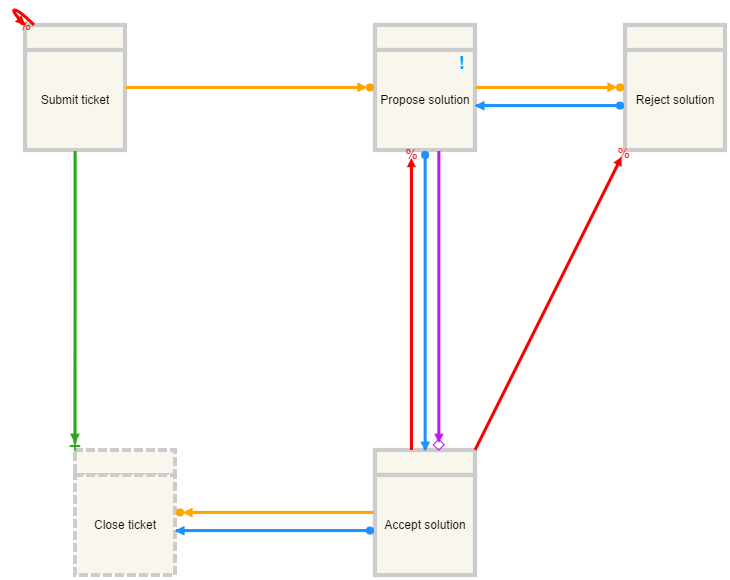
\includegraphics[scale=0.45]{figures/ExampleWorkflow.png}

	\section{Multi-contract}

		\subsection{Code}

			\lstinputlisting[language=solidity]{../contracts/workflow.sol}

		\subsection{Costs}

			\begin{tabular}{| l | l |}
				\hline
				Action & Cost (gas) \\ \hline
				Contract creation & 0 \\
				\hline
			\end{tabular}

	\section{Mono-contract}

		\subsection{Code}

			\lstinputlisting[language=solidity]{../contracts/monolith.sol}

		\subsection{Costs}

			\begin{tabular}{| l | l |}
				\hline
				Action & Cost (gas) \\ \hline
				Contract creation & 0 \\
				\hline
			\end{tabular}

\end{document}